\documentclass[11pt,a4paper]{article}

% ---------- Paquets ----------
\usepackage[utf8]{inputenc}
\usepackage[T1]{fontenc}
\usepackage[french]{babel}
\usepackage{lmodern}
\usepackage[margin=2.5cm]{geometry}
\usepackage{amsmath,amssymb}
\usepackage{icomma}
\usepackage{graphicx}
\usepackage{float}
\usepackage{caption}
\usepackage{subcaption}
\usepackage{array}
\usepackage{xcolor}
\usepackage{tikz}
\usepackage[hidelinks]{hyperref}

\definecolor{orangeesir}{RGB}{230,120,40}
\graphicspath{{images/}}
\renewcommand{\arraystretch}{1.25}

\begin{document}

% =====================================================================
%                          PAGE DE GARDE
% =====================================================================
\pagenumbering{gobble}
\begin{titlepage}
\begin{tikzpicture}[remember picture,overlay]
  \draw[line width=0.6pt]
    ([xshift=2cm,yshift=-2cm]current page.north west)
    rectangle
    ([xshift=-2cm,yshift=2cm]current page.south east);
\end{tikzpicture}

\centering
\vspace*{0.3cm}


\includegraphics[width=0.45\textwidth]{logo_univ_rennes.png}

\vspace{1cm}


\includegraphics[width=0.22\textwidth]{logo esir.png}

\vspace{3cm}

{\Large\bfseries \underline{Travaux Pratiques 2 :} Transformée de Fourier rapide\par}
\vspace{0.3cm}
{\large Partie 2 : analyse fréquentielle et compression d'images\par}
\vspace{0.3cm}
Algorithmique et Complexité, ESIR 2 IOT

\vspace{3cm}

\begin{minipage}[t]{0.42\textwidth}
  \centering
  {\color{orangeesir}\bfseries PROFESSEUR}\\[0.3cm]
  \fbox{\parbox[c][2cm][c]{0.9\linewidth}{\centering M. Pierre MAUREL}}
\end{minipage}
\hfill
\begin{minipage}[t]{0.42\textwidth}
  \centering
  {\color{orangeesir}\bfseries ÉTUDIANTS}\\[0.3cm]
  \fbox{\parbox[c][2cm][c]{0.9\linewidth}{\centering
    COULIBALY Yaplé Assétou\\[0.2cm]
    KOUAKOU Yah Mardochée}}
\end{minipage}

\vfill

\fbox{\parbox{0.6\textwidth}{\centering\bfseries\itshape ANNÉE ACADÉMIQUE : 2026-2027}}

\vspace{0.5cm}
\end{titlepage}

\pagenumbering{roman}
\tableofcontents
\newpage
\pagenumbering{arabic}

% =====================================================================

% =====================================================================
\section{Introduction}
% =====================================================================

Dans cette partie, on a utilisé notre FFT de la partie 1 pour calculer des spectres,
d'abord sur des signaux 1D, puis sur des images avec la TFD 2D fournie. On a ensuite
testé les deux méthodes de compression de l'énoncé (carré de basses fréquences et
seuillage) et on les a comparées. Pour chaque expérience, on a écrit ce qu'on
s'attendait à obtenir avant de lancer le calcul.

% =====================================================================
\section{TFD d'un signal 1D}
% =====================================================================

On a calculé la TFD des signaux de l'exercice 1 ($n = 16$). Les coefficients qui ne
sont pas cités dans le tableau sont nuls ; on obtient en fait des valeurs de l'ordre
de $10^{-15}$, qui sont des erreurs d'arrondi.

\begin{table}[H]
\centering
\caption{TFD de signaux de taille $n = 16$ : prévision et résultat.}
\label{tab:1d}
\begin{tabular}{|l|l|c|}
\hline
\textbf{Signal $a_t$} & \textbf{Prévision} & \textbf{Résultat} \\
\hline
constante $c = 3$ ; $-2$ ; $0{,}5$ & $y_0 = 16c = 48$ ; $-32$ ; $8$ & conforme \\
\hline
$\cos(2\pi k t/n)$, $0 < k < 8$ & $y_k = y_{16-k} = 8$ & conforme \\
\hline
$\cos(2\pi k t/n)$, $k = 0$ ou $k = 8$ & un seul pic $y_k = 16$ & conforme \\
\hline
$\cos(2\pi k t/n)$, $8 < k < 16$ & même TFD que pour $16-k$ & conforme \\
\hline
$\cos(2\pi t/n) + \frac12 \cos(2\pi\, 3t/n)$ & $y_1 = y_{15} = 8$, $y_3 = y_{13} = 4$ & conforme \\
\hline
$4 + 2\sin(2\pi\, 2t/n) + \cos(2\pi\, 7t/n)$ &
  $y_0 = 64$, $y_2 = 16i$, $y_{14} = -16i$, $y_7 = y_9 = 8$ & conforme \\
\hline
\end{tabular}
\end{table}

Toutes nos prévisions sont vérifiées. Ce qu'on en retient :
\begin{itemize}
  \item \textbf{Constante.} $y_0$ est la somme des valeurs ($n \times$ moyenne). Les
        autres coefficients sont nuls car $y_k = c \sum_j \omega_n^{kj}$ est une somme
        de racines de l'unité.
  \item \textbf{Cosinus.} Deux pics de $A\,n/2$, en $k$ et $n-k$ (décomposition donnée
        dans l'énoncé). Pour $k = 0$ et $k = 8$, les deux indices sont les mêmes, donc
        un seul pic de 16.
  \item \textbf{$k > 8$.} On obtient exactement le spectre de $16-k$ : aux instants
        entiers, $\cos(2\pi k t/n) = \cos(2\pi (n-k) t/n)$, ce sont les mêmes
        échantillons. Avec 16 points, on ne peut pas voir de fréquence au-dessus de 8
        (repliement, Shannon).
  \item \textbf{Somme.} La TFD est linéaire, les deux spectres s'ajoutent (le
        $\frac12$ donne des pics de 4).
  \item \textbf{Sinus.} Les pics sont imaginaires et de signes opposés ($+16i$ en 2,
        $-16i$ en 14), parce que $\sin\theta = (e^{i\theta} - e^{-i\theta})/2i$.
\end{itemize}

% =====================================================================
\section{TFD d'une image}
% =====================================================================

\subsection{Vérification de la TFD 2D}

On a appliqué la TFD puis la TFD inverse à l'image du tigre ($512 \times 512$). On
retrouve la même image : l'écart maximal sur les pixels est de $1{,}1\cdot10^{-13}$ niveau de gris, donc
seulement des erreurs d'arrondi. Ça valide aussi notre FFT 1D, que la TFD 2D utilise sur chaque ligne et
chaque colonne ($2n$ FFT de taille $n$, donc un coût en $\Theta(n^2 \log n)$).

Au premier essai, on avait appliqué deux fois la TFD au lieu de la TFD puis
l'inverse. On obtenait le tigre retourné de $180^\circ$ avec les quatre quarts de
l'image échangés : deux TFD de suite retournent l'image, et le recentrage, fait à
chaque TFD, décale de $n/2$, ce qui échange les quarts.

\subsection{Affichage d'un spectre}
\label{sec:affichage}

Le module de la TFD est énorme au centre (il vaut $n \times$ la moyenne de l'image)
et très petit ailleurs. Comme l'enregistrement coupe à 255, on ne verrait que le
centre. On a donc écrit une fonction qui affiche $\log(1 + |F|)$, ramené entre 0 et
255 en multipliant par $255 / \max$. Le logarithme rapproche les grandes et les
petites valeurs, et le $1+$ évite $\log 0$. Tous les spectres sont affichés comme ça
(figure~\ref{fig:log}).

\begin{figure}[H]
\centering
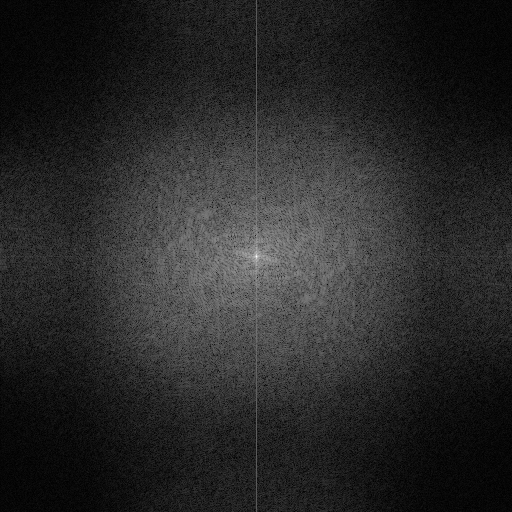
\includegraphics[width=0.32\textwidth]{spectre_tigre_log.png}
\caption{Module de la TFD du tigre, affiché avec $\log(1 + |F|)$.}
\label{fig:log}
\end{figure}

\subsection{Spectres des mires, de l'empreinte et de barbara}

On a fait nos prévisions avec la règle de l'énoncé : des rayures donnent deux points
symétriques, dans la direction perpendiculaire aux rayures, et d'autant plus loin du
centre que les rayures sont fines. On a mesuré la position des points en pixels à
partir du centre ; pour une sinusoïde, elle donne le nombre de périodes sur la taille
de l'image.

\begin{table}[H]
\centering
\caption{Spectres : prévision et observation (positions en pixels depuis le centre).}
\label{tab:spectres}
\begin{tabular}{|l|p{5.3cm}|p{6.2cm}|}
\hline
\textbf{Image} & \textbf{Prévision} & \textbf{Observation} \\
\hline
mire1 & deux points symétriques sur l'axe horizontal &
  points à $\pm 4$ sur l'axe horizontal : rayures verticales, 4 périodes sur la largeur \\
\hline
mire2 & même chose, plus loin du centre (rayures plus serrées) &
  points à $\pm 8$ sur l'axe horizontal : 8 périodes \\
\hline
mire3 & points hors des axes, par paires symétriques &
  deux paires : $(0, \pm 5)$ et $\pm(20, -10)$ (colonne, ligne), donc deux ondes
  superposées \\
\hline
fingerprint & un anneau centré & un anneau, plus une croix faible sur les axes \\
\hline
barbara & centre brillant, croix sur les axes, taches isolées dues aux rayures &
  conforme, avec des taches allongées dans des directions obliques \\
\hline
\end{tabular}
\end{table}

\begin{figure}[H]
\centering
\begin{tabular}{ccc}
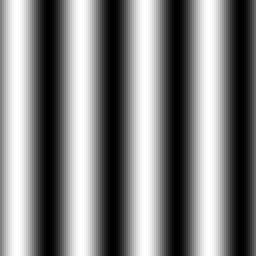
\includegraphics[width=0.27\textwidth]{mire1.png} &
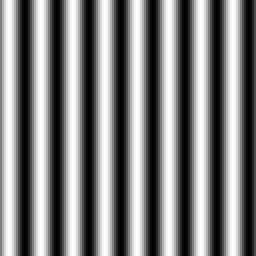
\includegraphics[width=0.27\textwidth]{mire2.png} &
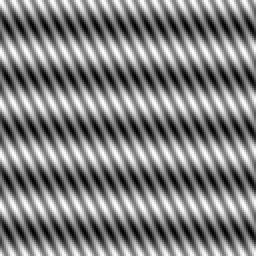
\includegraphics[width=0.27\textwidth]{mire3.png} \\
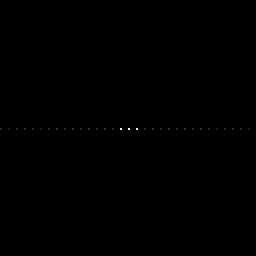
\includegraphics[width=0.27\textwidth]{spectre_mire1.png} &
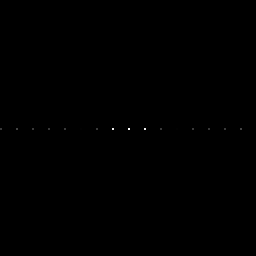
\includegraphics[width=0.27\textwidth]{spectre_mire2.png} &
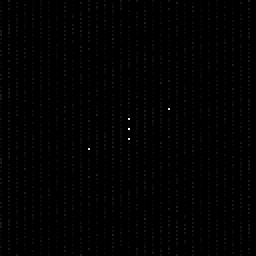
\includegraphics[width=0.27\textwidth]{spectre_mire3.png} \\
mire1 & mire2 & mire3
\end{tabular}
\caption{Mires ($128 \times 128$) et module de leur TFD (échelle logarithmique).}
\label{fig:mires}
\end{figure}

\begin{figure}[H]
\centering
\begin{tabular}{cc}
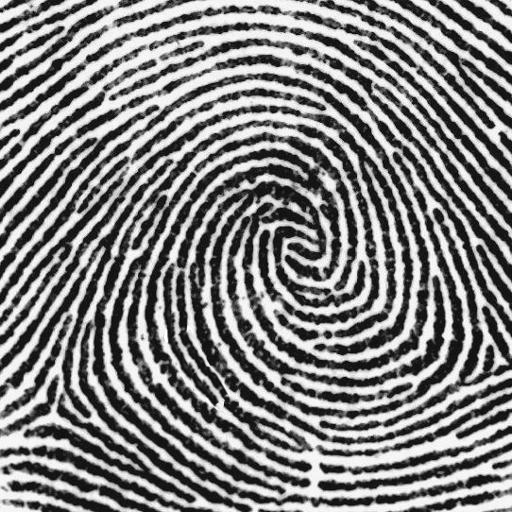
\includegraphics[width=0.36\textwidth]{fingerprint.png} &
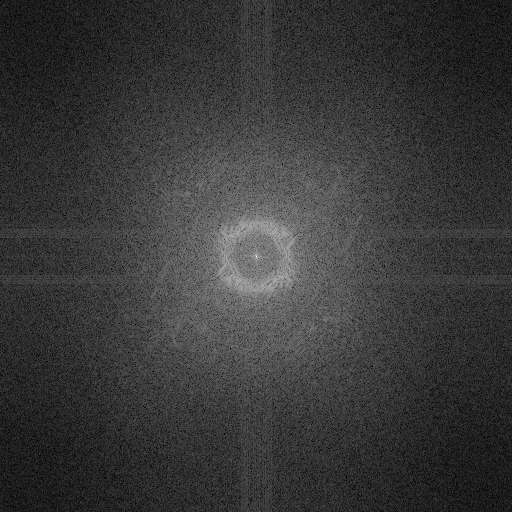
\includegraphics[width=0.36\textwidth]{spectre_fingerprint.png} \\
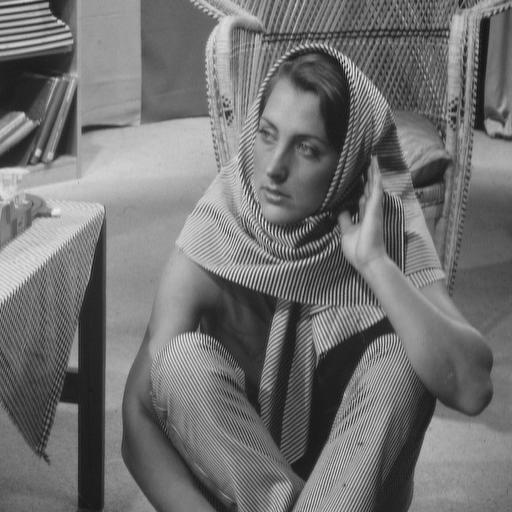
\includegraphics[width=0.36\textwidth]{barbara.png} &
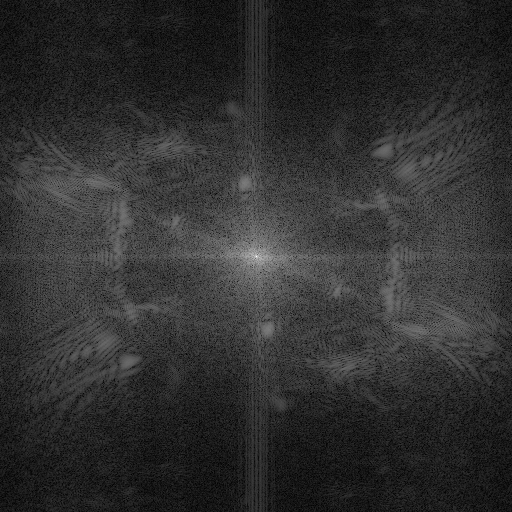
\includegraphics[width=0.36\textwidth]{spectre_barbara.png}
\end{tabular}
\caption{Empreinte et barbara ($512 \times 512$) avec le module de leur TFD.}
\label{fig:fp-barbara}
\end{figure}

Ce qu'on a observé :
\begin{itemize}
  \item \textbf{mire1, mire2.} 4 puis 8 périodes sur la largeur, donc des points à 4
        puis 8 pixels du centre. Par contre, on n'avait pas prévu la ligne de petits
        points sur l'axe horizontal, tous les 4 pixels (mire1) ou 8 pixels (mire2). On
        pense qu'elle vient de l'arrondi des pixels à des entiers : la mire n'est pas
        une sinusoïde exacte. Cette erreur est la même sur toutes les lignes de
        l'image, donc elle ne peut donner des points que sur l'axe horizontal, et elle
        se répète avec la période des rayures, donc tous les 4 (ou 8) pixels. Ces
        coefficients sont minuscules, on ne les voit que grâce au logarithme.
  \item \textbf{mire3.} Il y a deux paires de points, donc l'image est la somme de
        deux ondes : des rayures horizontales (5 périodes sur la hauteur)
        et des rayures obliques (point en $(20, -10)$, soit
        $\sqrt{20^2 + 10^2} \approx 22$ périodes).
  \item \textbf{Empreinte.} Les crêtes sont à peu près toutes espacées pareil mais
        tournent dans toutes les directions : un point par direction, à la même
        distance du centre, ce qui fait un anneau. Le fond gris vient des contours
        noir/blanc très nets (hautes fréquences).
  \item \textbf{Barbara.} Les taches loin du centre correspondent aux rayures du
        foulard, du pantalon et de la nappe, qui n'ont pas la même orientation.
  \item \textbf{Croix sur les axes.} On la voit pour l'empreinte, barbara et le tigre,
        pas pour les mires. Notre explication : la TFD traite l'image comme si elle se
        répétait, donc le bord droit touche le bord gauche ; sur une photo les deux
        bords sont différents, ce qui fait comme un contour vertical (et pareil en
        haut et en bas). Les mires ont un nombre entier de périodes, leurs bords se
        raccordent.
\end{itemize}

% =====================================================================
\section{Compression d'images}
% =====================================================================

\subsection{Annulation d'un seul coefficient}

On a annulé un coefficient de la TFD du tigre puis calculé la TFD inverse, en
repartant à chaque fois de la TFD complète. Pour chaque cas, on a mesuré l'écart
maximal entre l'image obtenue et l'originale.

\begin{table}[H]
\centering
\caption{Annulation d'un coefficient de la TFD du tigre ($n = 512$).}
\label{tab:ex4}
\begin{tabular}{|c|p{2.2cm}|p{4cm}|p{4.5cm}|}
\hline
\textbf{Coefficient} & \textbf{Écart max (niv. de gris)} & \textbf{Prévision} & \textbf{Observation} \\
\hline
$(n/2, n/2)$ & 84,4 &
  moyenne retirée ; zones proches de la moyenne noires & conforme
  (figure~\ref{fig:ex4}a) \\
\hline
$(n/2+1, n/2)$ & 20,2 &
  image quasi identique, léger dégradé & identique à l'\oe il ; écart : un dégradé
  vertical d'une période \\
\hline
$(n/2+100, n/2)$ & 0,16 & image inchangée & conforme ; écart : fines lignes
  horizontales \\
\hline
\end{tabular}
\end{table}

\begin{figure}[H]
\centering
\begin{subfigure}{0.3\textwidth}\centering
  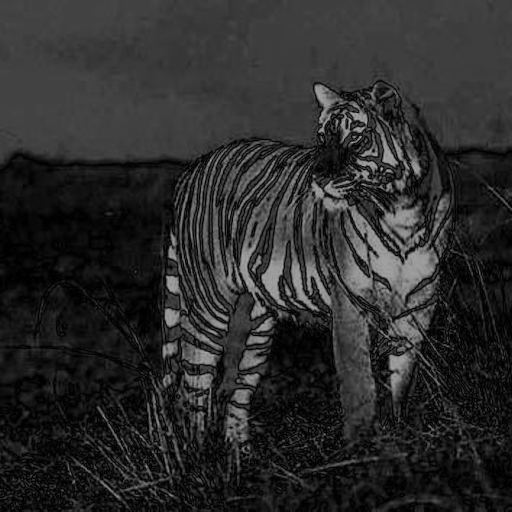
\includegraphics[width=\linewidth]{ex4_centre.png}
  \caption{centre annulé}
\end{subfigure}
\hfill
\begin{subfigure}{0.3\textwidth}\centering
  
\includegraphics[width=\linewidth]{ex4_diff_voisin.png}
  \caption{écart, $(n/2+1, n/2)$}
\end{subfigure}
\hfill
\begin{subfigure}{0.3\textwidth}\centering
  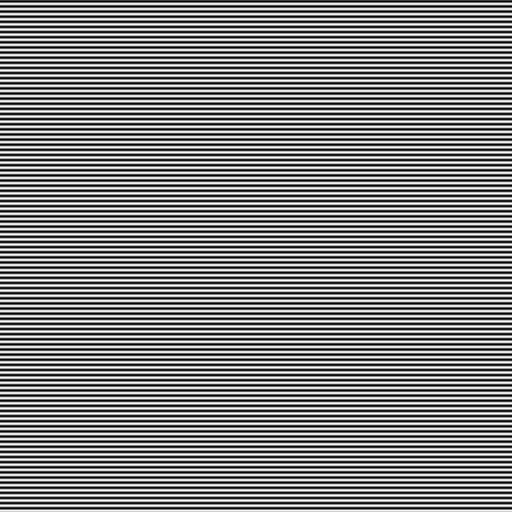
\includegraphics[width=\linewidth]{ex4_diff_HF.png}
  \caption{écart, $(n/2+100, n/2)$}
\end{subfigure}
\caption{Annulation d'un coefficient. Pour (b) et (c), l'image montre la différence
avec l'original, contraste étiré (gris moyen = 0).}
\label{fig:ex4}
\end{figure}

\begin{itemize}
  \item \textbf{Centre.} Comme prévu, on retire la moyenne : l'image vaut
        $I - 84{,}4$, avec des valeurs négatives. Comme on enregistre le module, on
        voit $|I - 84{,}4|$ : l'herbe, proche de la moyenne, devient noire, le ciel
        sombre devient gris, les rayures noires deviennent claires.
  \item \textbf{Voisin du centre.} L'écart est de 20 niveaux de gris, plus que ce
        qu'on pensait, mais on ne voit aucune différence : c'est un dégradé d'une seule
        période sur toute la hauteur (figure~\ref{fig:ex4}b), trop lent pour l'\oe il.
  \item \textbf{Haute fréquence.} 0,16 niveau de gris d'écart : invisible, comme
        prévu.
\end{itemize}
Le centre donne la luminosité moyenne, les coefficients proches les grandes
variations, ceux qui sont loin les détails fins, et ces derniers sont petits. C'est
ce qui permet de compresser.

\subsection{Compression par sélection des basses fréquences}

Dans notre fonction, les indices gardés vont de $n/2-k+1$ à $n/2+k$ ($2k$ valeurs) ;
le carré n'est donc pas tout à fait symétrique, mais ça ne change rien de visible.

\begin{table}[H]
\centering
\caption{Compression du tigre par un carré de côté $2k$ ($512^2 = 262\,144$
coefficients au total).}
\label{tab:ex5}
\begin{tabular}{|r|r|r|}
\hline
$k$ & \textbf{Coefficients gardés} & \textbf{Fraction} \\
\hline
4   & 64      & 0,024\,\% \\
\hline
8   & 256     & 0,098\,\% \\
\hline
16  & 1\,024  & 0,39\,\%  \\
\hline
32  & 4\,096  & 1,56\,\%  \\
\hline
64  & 16\,384 & 6,25\,\%  \\
\hline
128 & 65\,536 & 25\,\%    \\
\hline
\end{tabular}
\end{table}

\begin{figure}[H]
\centering
\begin{tabular}{ccc}
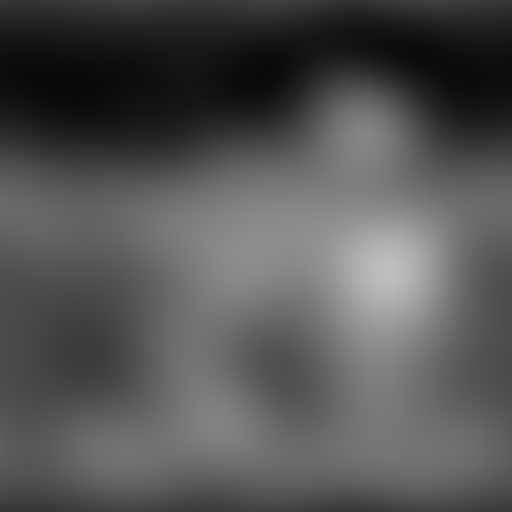
\includegraphics[width=0.3\textwidth]{ex5_k4.png} &
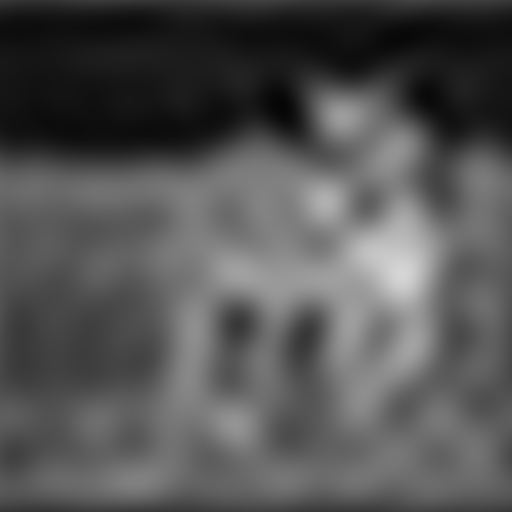
\includegraphics[width=0.3\textwidth]{ex5_k8.png} &
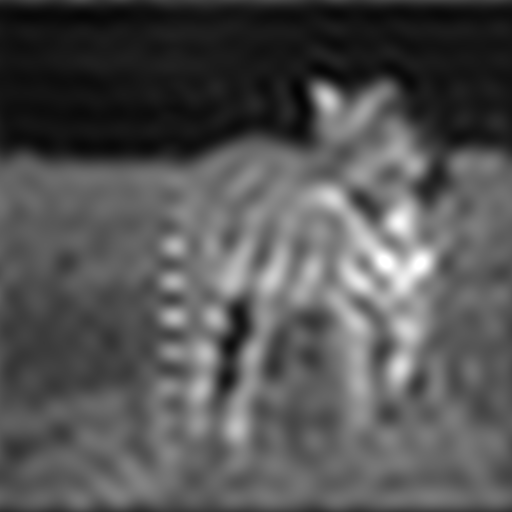
\includegraphics[width=0.3\textwidth]{ex5_k16.png} \\
$k = 4$ & $k = 8$ & $k = 16$ \\[0.2cm]
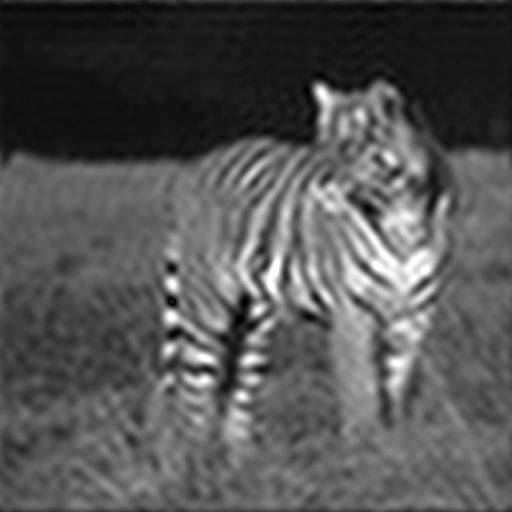
\includegraphics[width=0.3\textwidth]{ex5_k32.png} &
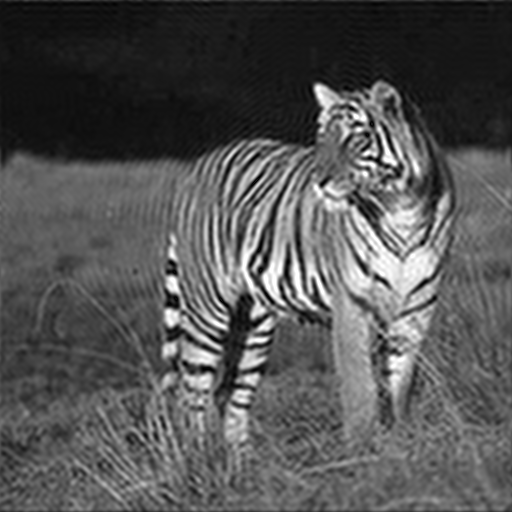
\includegraphics[width=0.3\textwidth]{ex5_k64.png} &
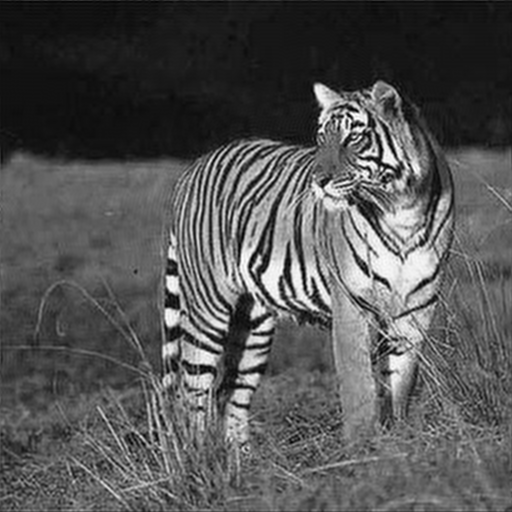
\includegraphics[width=0.3\textwidth]{ex5_k128.png} \\
$k = 32$ & $k = 64$ & $k = 128$
\end{tabular}
\caption{Tigre reconstruit à partir du carré de basses fréquences de côté $2k$.}
\label{fig:ex5}
\end{figure}

\begin{table}[H]
\centering
\caption{Compression par carré : prévision et observation.}
\label{tab:ex5prev}
\begin{tabular}{|c|p{6cm}|p{6cm}|}
\hline
$k$ & \textbf{Prévision} & \textbf{Observation} \\
\hline
4 & très floue, à peine reconnaissable & conforme : taches floues \\
\hline
16 & reconnaissable & conforme : silhouette et rayures floues \\
\hline
32 & floue, formes reconnaissables, oscillations près des contours &
  conforme : rayures nettes, herbe floue, ondulations près des contours \\
\hline
64 & visuellement bonne & conforme : seul le détail de l'herbe est perdu \\
\hline
128 & pas de différence nette & conforme : presque identique à l'original \\
\hline
\end{tabular}
\end{table}

Nos prévisions sont vérifiées. Le flou vient des hautes fréquences supprimées. Les
ondulations autour des contours (bien visibles à $k = 32$) sont le phénomène de
Gibbs : un contour net a besoin de toutes les fréquences, et on les coupe d'un coup à
$k$.

\subsection{Compression par seuillage}

On a testé notre fonction de seuillage sur le tigre avec un seuil de 30 : elle garde
30\,808 coefficients sur 262\,144, soit 11,8\,\%. Avec un seuil assez petit, on
garde donc déjà très peu de coefficients : la plupart sont petits. Ce test nous a
aussi donné l'ordre de grandeur du seuil pour l'exercice 7.

\subsection{\texorpdfstring{Comparaison des deux méthodes à 10\,\%}{Comparaison des deux méthodes à 10 \%}}

\paragraph{Ce qu'on a fait.} Pour le carré, on a pris $k = 81$, soit
$(2 \times 81)^2 = 26\,244$ coefficients (10,01\,\%). Pour le seuil, il fallait
trouver la valeur qui garde le même nombre de coefficients. Comme ce nombre diminue
quand le seuil augmente, on l'a cherché par dichotomie entre 0 et 200\,000 (le plus
grand coefficient ne peut pas dépasser $512 \times 255$), avec 40 itérations. À chaque
itération, on repart de la TFD complète, parce que notre fonction de seuillage modifie
le tableau. On a ensuite comparé les images, et calculé pour chaque méthode l'erreur
quadratique moyenne entre l'image $I$ et l'image reconstruite $I'$ :
\[
  \mathrm{MSE} = \frac{1}{n^2} \sum_{k,l} \bigl(I(k,l) - I'(k,l)\bigr)^2 .
\]

\begin{table}[H]
\centering
\caption{Comparaison carré / seuil, 26\,244 coefficients gardés (10\,\%).}
\label{tab:ex7}
\begin{tabular}{|l|l|r|r|r|}
\hline
\textbf{Image} & \textbf{Méthode} & \textbf{Gardés} & \textbf{Seuil} & \textbf{MSE (niv. de gris$^2$)} \\
\hline
tigre   & carré, $k = 81$ & 26\,244 & -     & 135,7 \\
\hline
tigre   & seuil           & 26\,244 & 35,6  & 74,0  \\
\hline
barbara & carré, $k = 81$ & 26\,244 & -     & 234,7 \\
\hline
barbara & seuil           & 26\,243 & 30,6  & 103,5 \\
\hline
\end{tabular}
\end{table}

\begin{figure}[H]
\centering
\begin{tabular}{ccc}
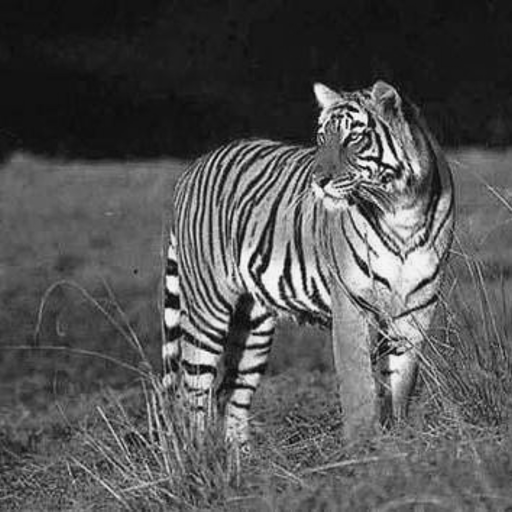
\includegraphics[width=0.3\textwidth]{tigre.png} &
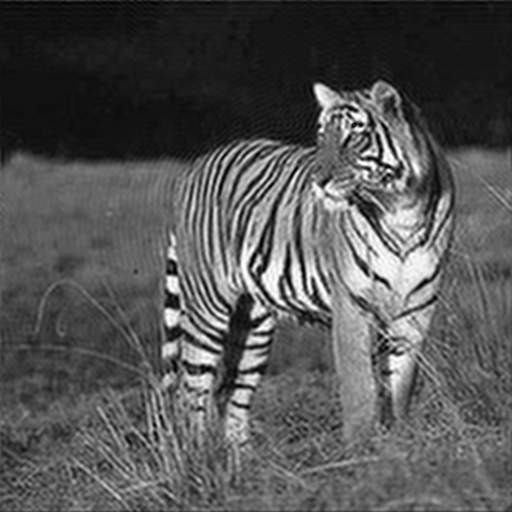
\includegraphics[width=0.3\textwidth]{ex7_tigre_carre.png} &
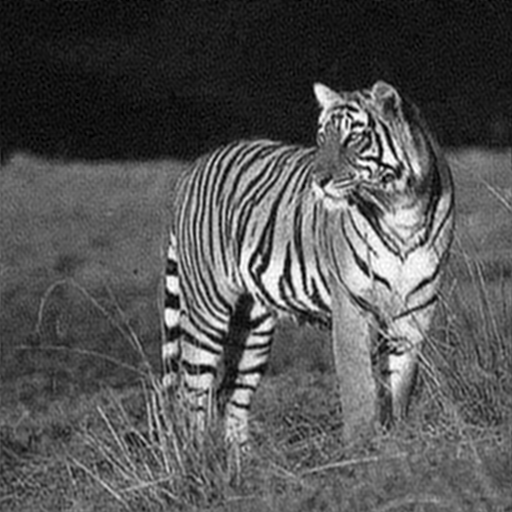
\includegraphics[width=0.3\textwidth]{ex7_tigre_seuil.png} \\
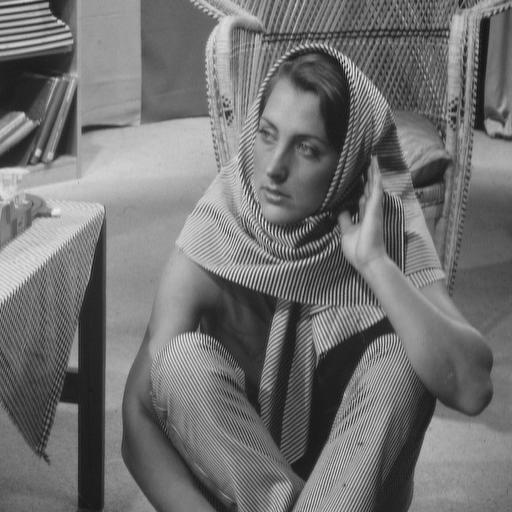
\includegraphics[width=0.3\textwidth]{barbara.png} &
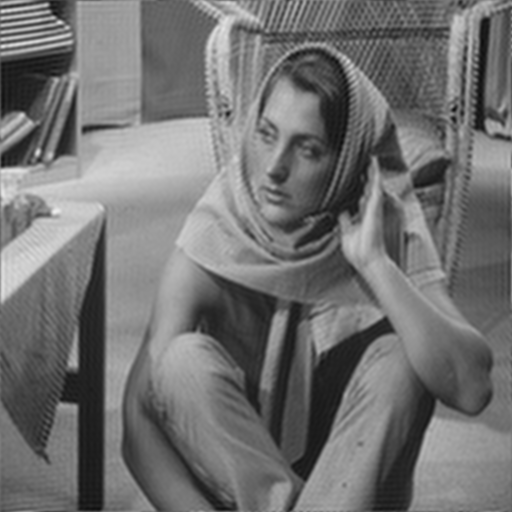
\includegraphics[width=0.3\textwidth]{ex7_barbara_carre.png} &
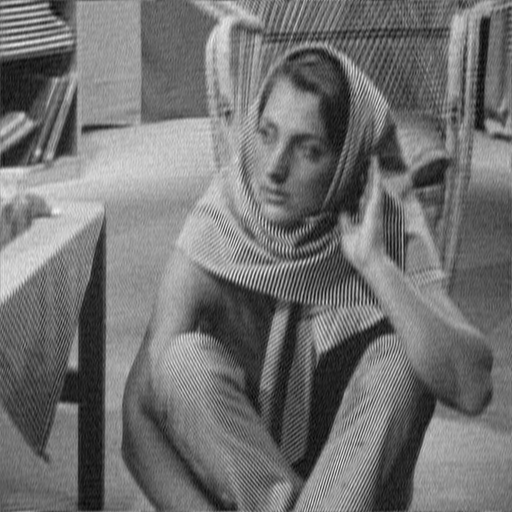
\includegraphics[width=0.3\textwidth]{ex7_barbara_seuil.png} \\
original & carré & seuil
\end{tabular}
\caption{Compression à 10\,\% des coefficients.}
\label{fig:ex7}
\end{figure}

\paragraph{Résultats.} Le seuil donne une MSE 1,8 fois plus faible pour le tigre et
2,3 fois pour barbara. Sur les images, le carré rend tout flou et efface les rayures
du pantalon et du foulard de barbara. Le seuil garde ces rayures, mais on voit un
léger grain dans les zones lisses.

\paragraph{Pourquoi le seuil est meilleur.} Avec le $1/n$, la TFD 2D conserve
l'énergie (Parseval), donc l'erreur vaut
\[
  \mathrm{MSE} = \frac{1}{n^2} \sum_{\text{coefficients annulés}} |F(u,v)|^2 .
\]
Pour un nombre de coefficients gardés fixé, cette somme est la plus petite
quand on annule les plus petits modules, et c'est exactement ce que fait le seuil.

L'écart est plus grand pour barbara : ses rayures sont des hautes fréquences avec un
grand module (les taches loin du centre de son spectre). Le carré les supprime, le
seuil les garde.

\paragraph{Limite.} Avec le carré, on sait où sont les coefficients gardés (il suffit
de $k$). Avec le seuil, il faudrait aussi stocker la position de chacun, donc à nombre
de coefficients égal, le fichier serait plus gros. La comparaison à 10\,\% des
coefficients avantage donc un peu le seuil.

% =====================================================================
\section{Conclusion}
% =====================================================================

Nos prévisions sur les spectres ont toutes été vérifiées ; les seuls détails qu'on
n'avait pas prévus (petits points des mires, deux ondes dans mire3) ont une
explication. L'annulation d'un coefficient montre que ceux qui sont loin du centre
sont petits et ne changent presque rien, ce qui permet de compresser. Le carré de basses fréquences donne une image reconnaissable
avec moins de 1\,\% des coefficients, mais floue. À 10\,\% des coefficients, le
seuillage donne une erreur 1,8 à 2,3 fois plus faible, ce qu'on explique avec
Parseval, surtout sur une image avec beaucoup de textures comme barbara. Son
inconvénient est qu'il faut stocker la position des coefficients gardés.

\end{document}
